\begin{figure}[H]
    \centering
    \begin{subfigure}[b]{0.09\textwidth}
        \centering
        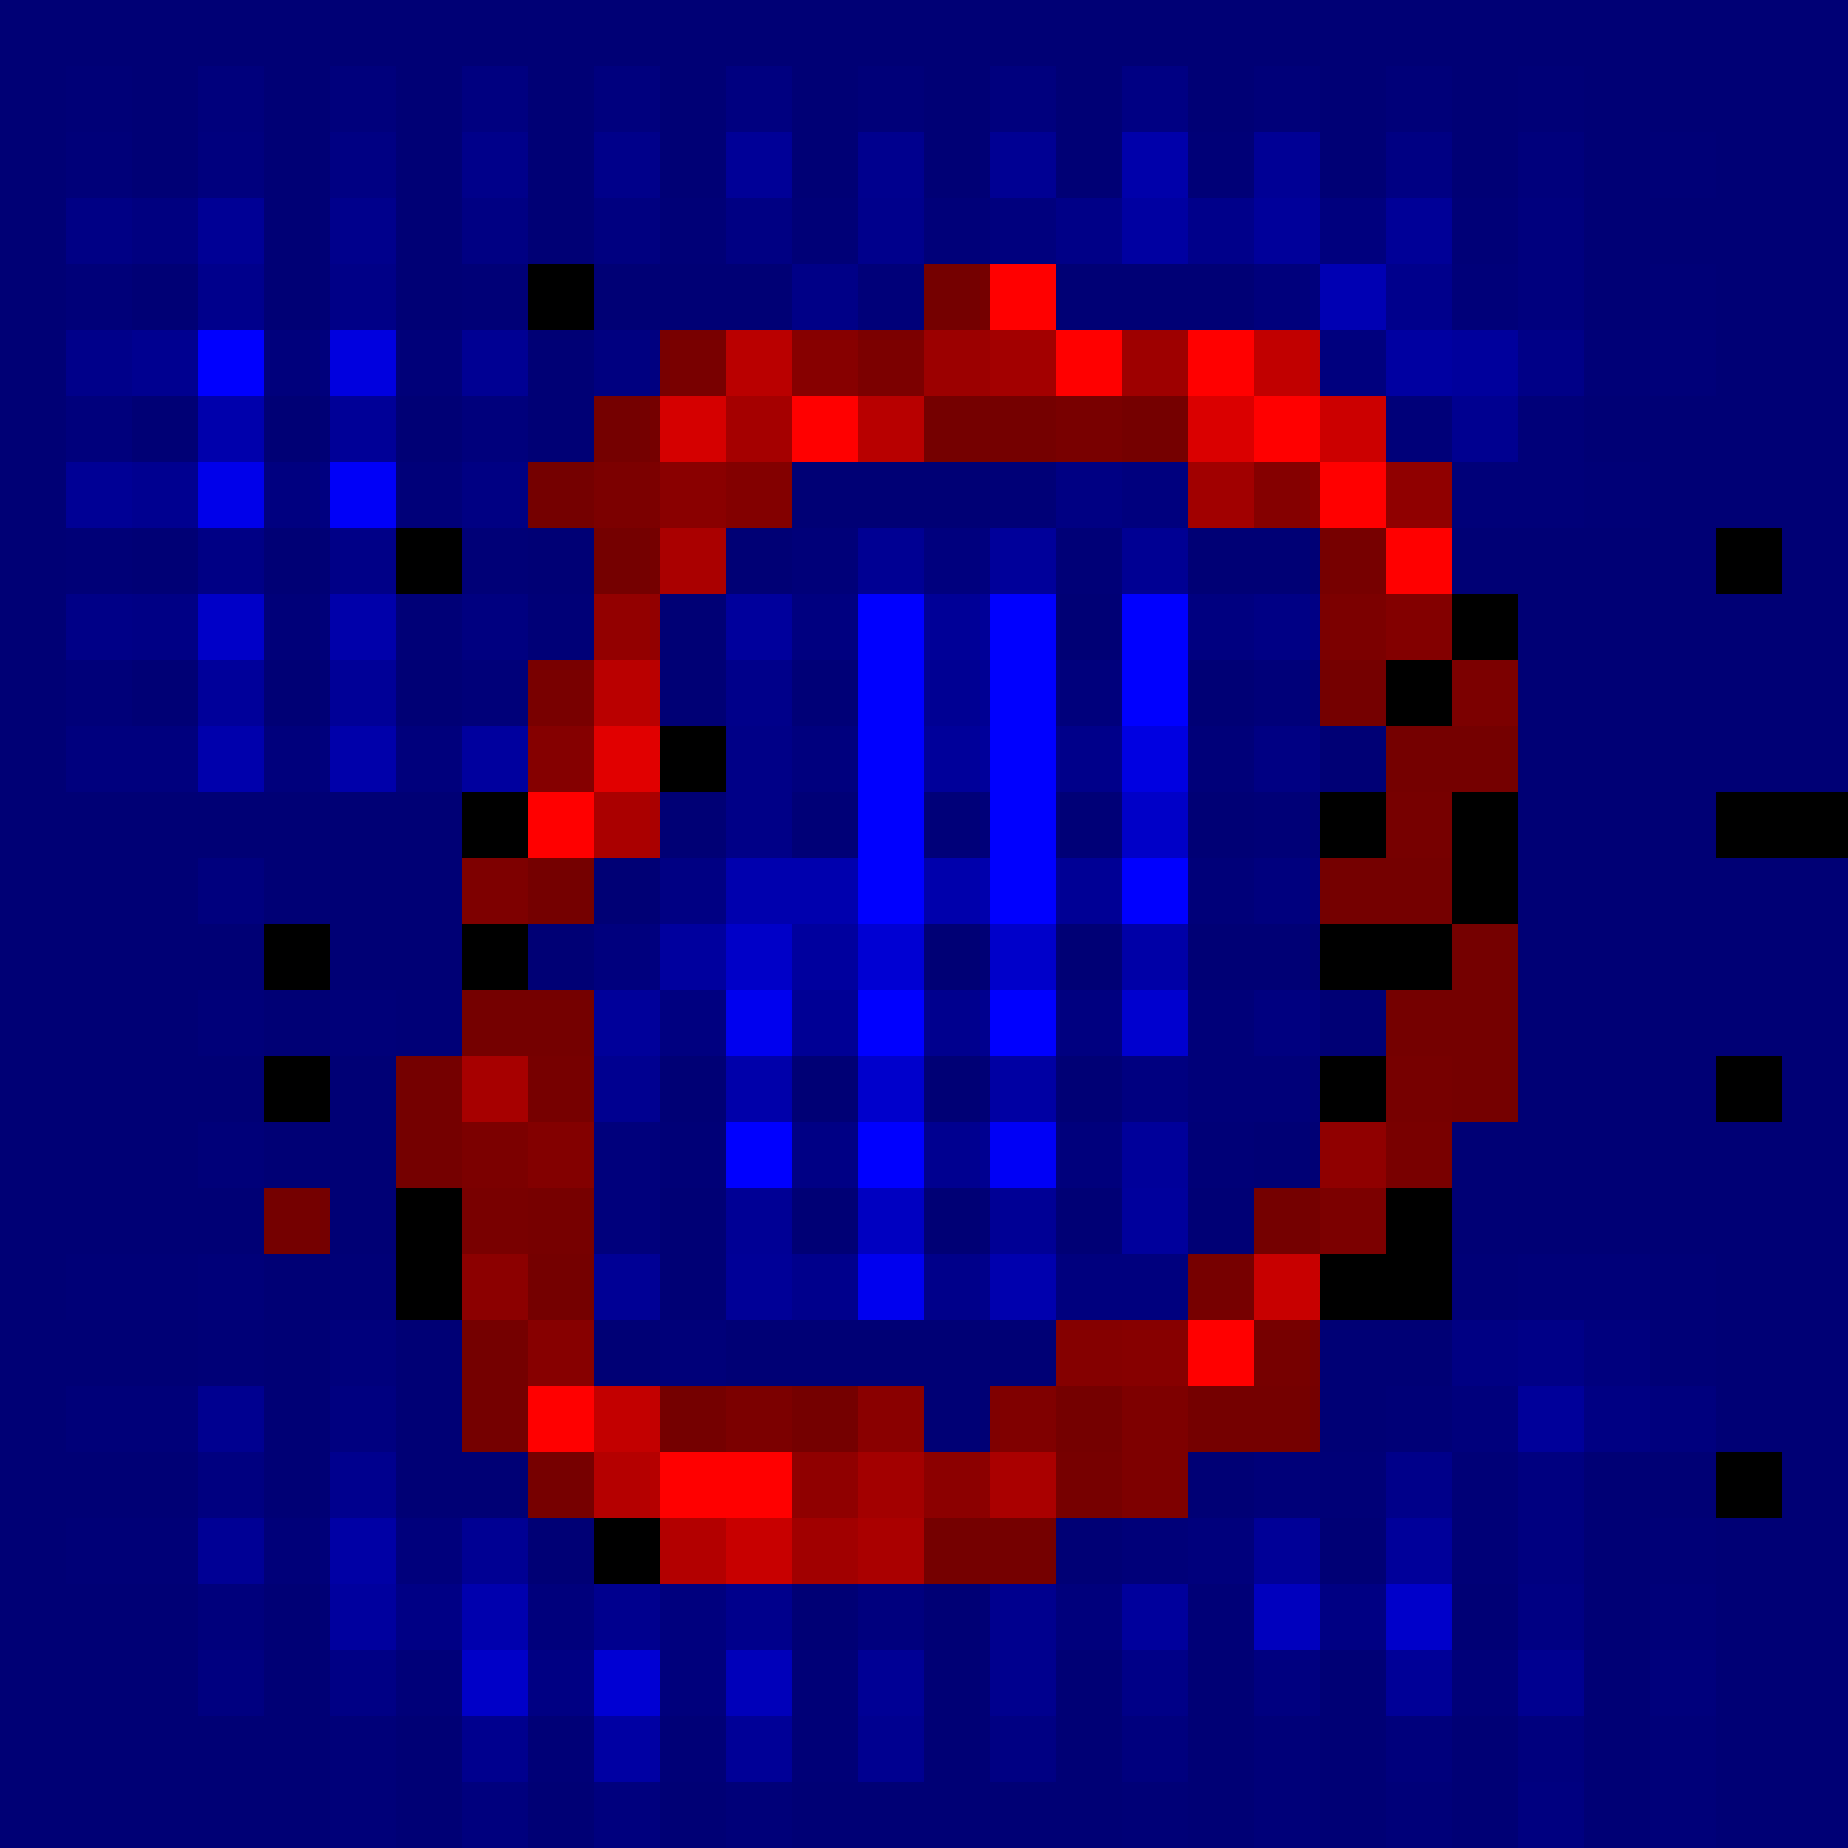
\includegraphics[width=\textwidth]{figures/mnist_ic_saliency/saliency_threshold_wrt_0_bright.png}
    \end{subfigure}
    \begin{subfigure}[b]{0.09\textwidth}
        \centering
        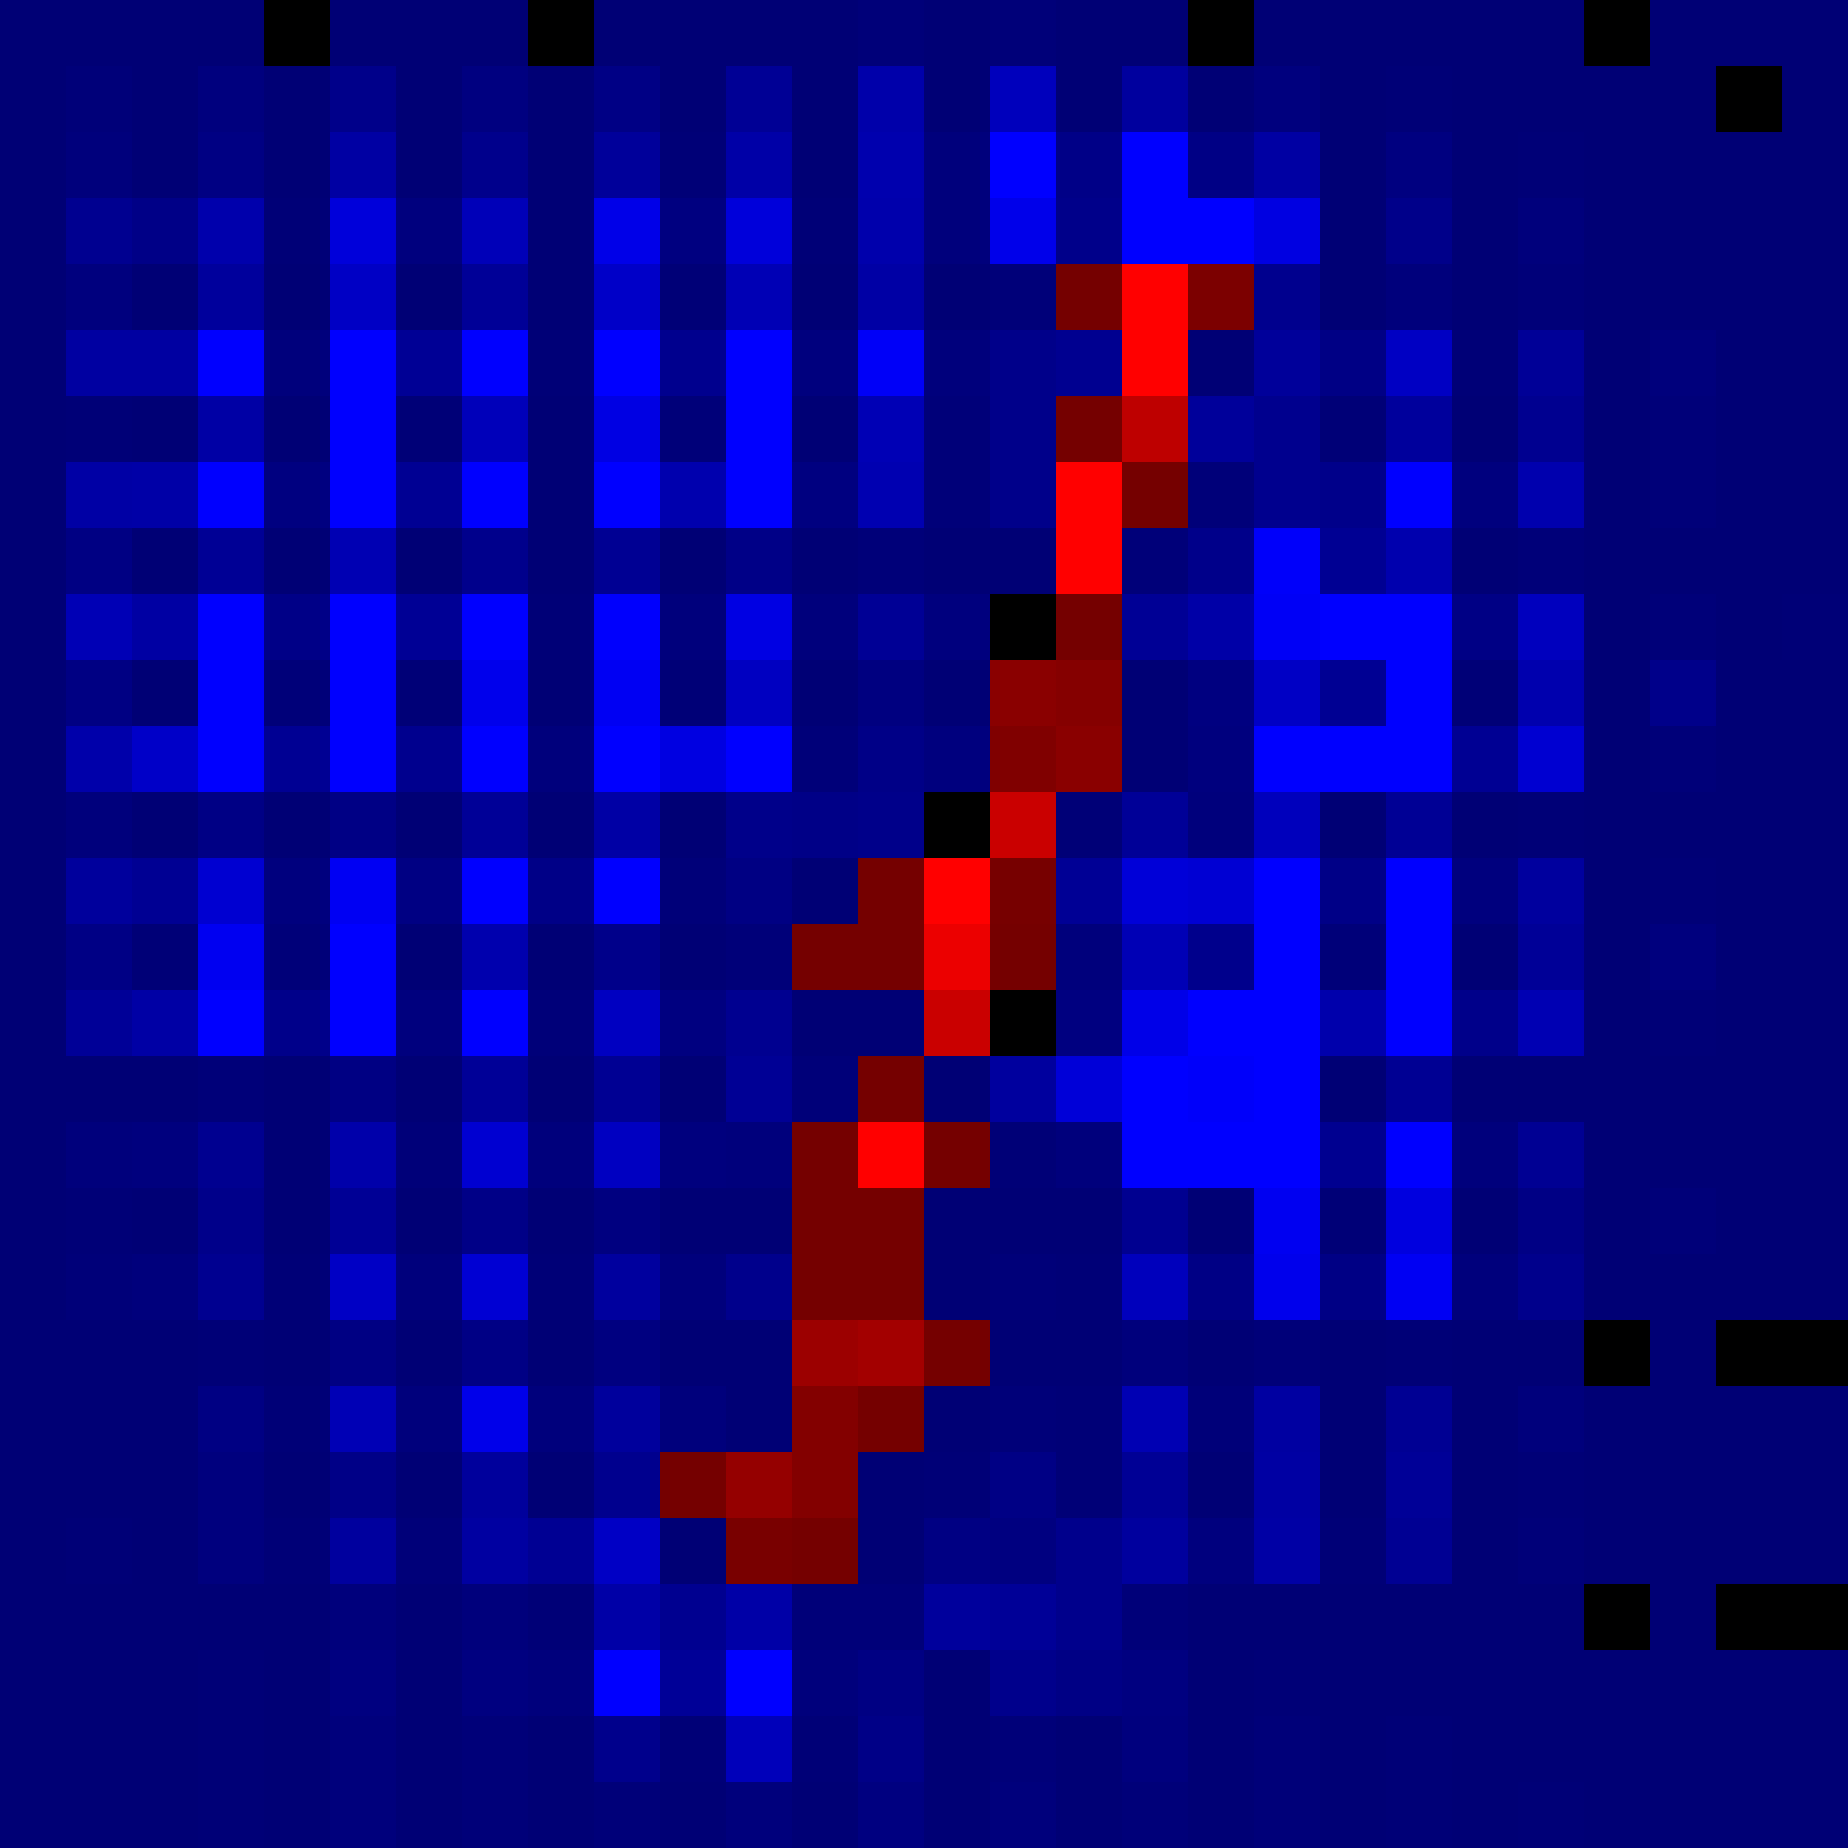
\includegraphics[width=\textwidth]{figures/mnist_ic_saliency/saliency_threshold_wrt_1_bright.png}
    \end{subfigure}
    \begin{subfigure}[b]{0.09\textwidth}
        \centering
        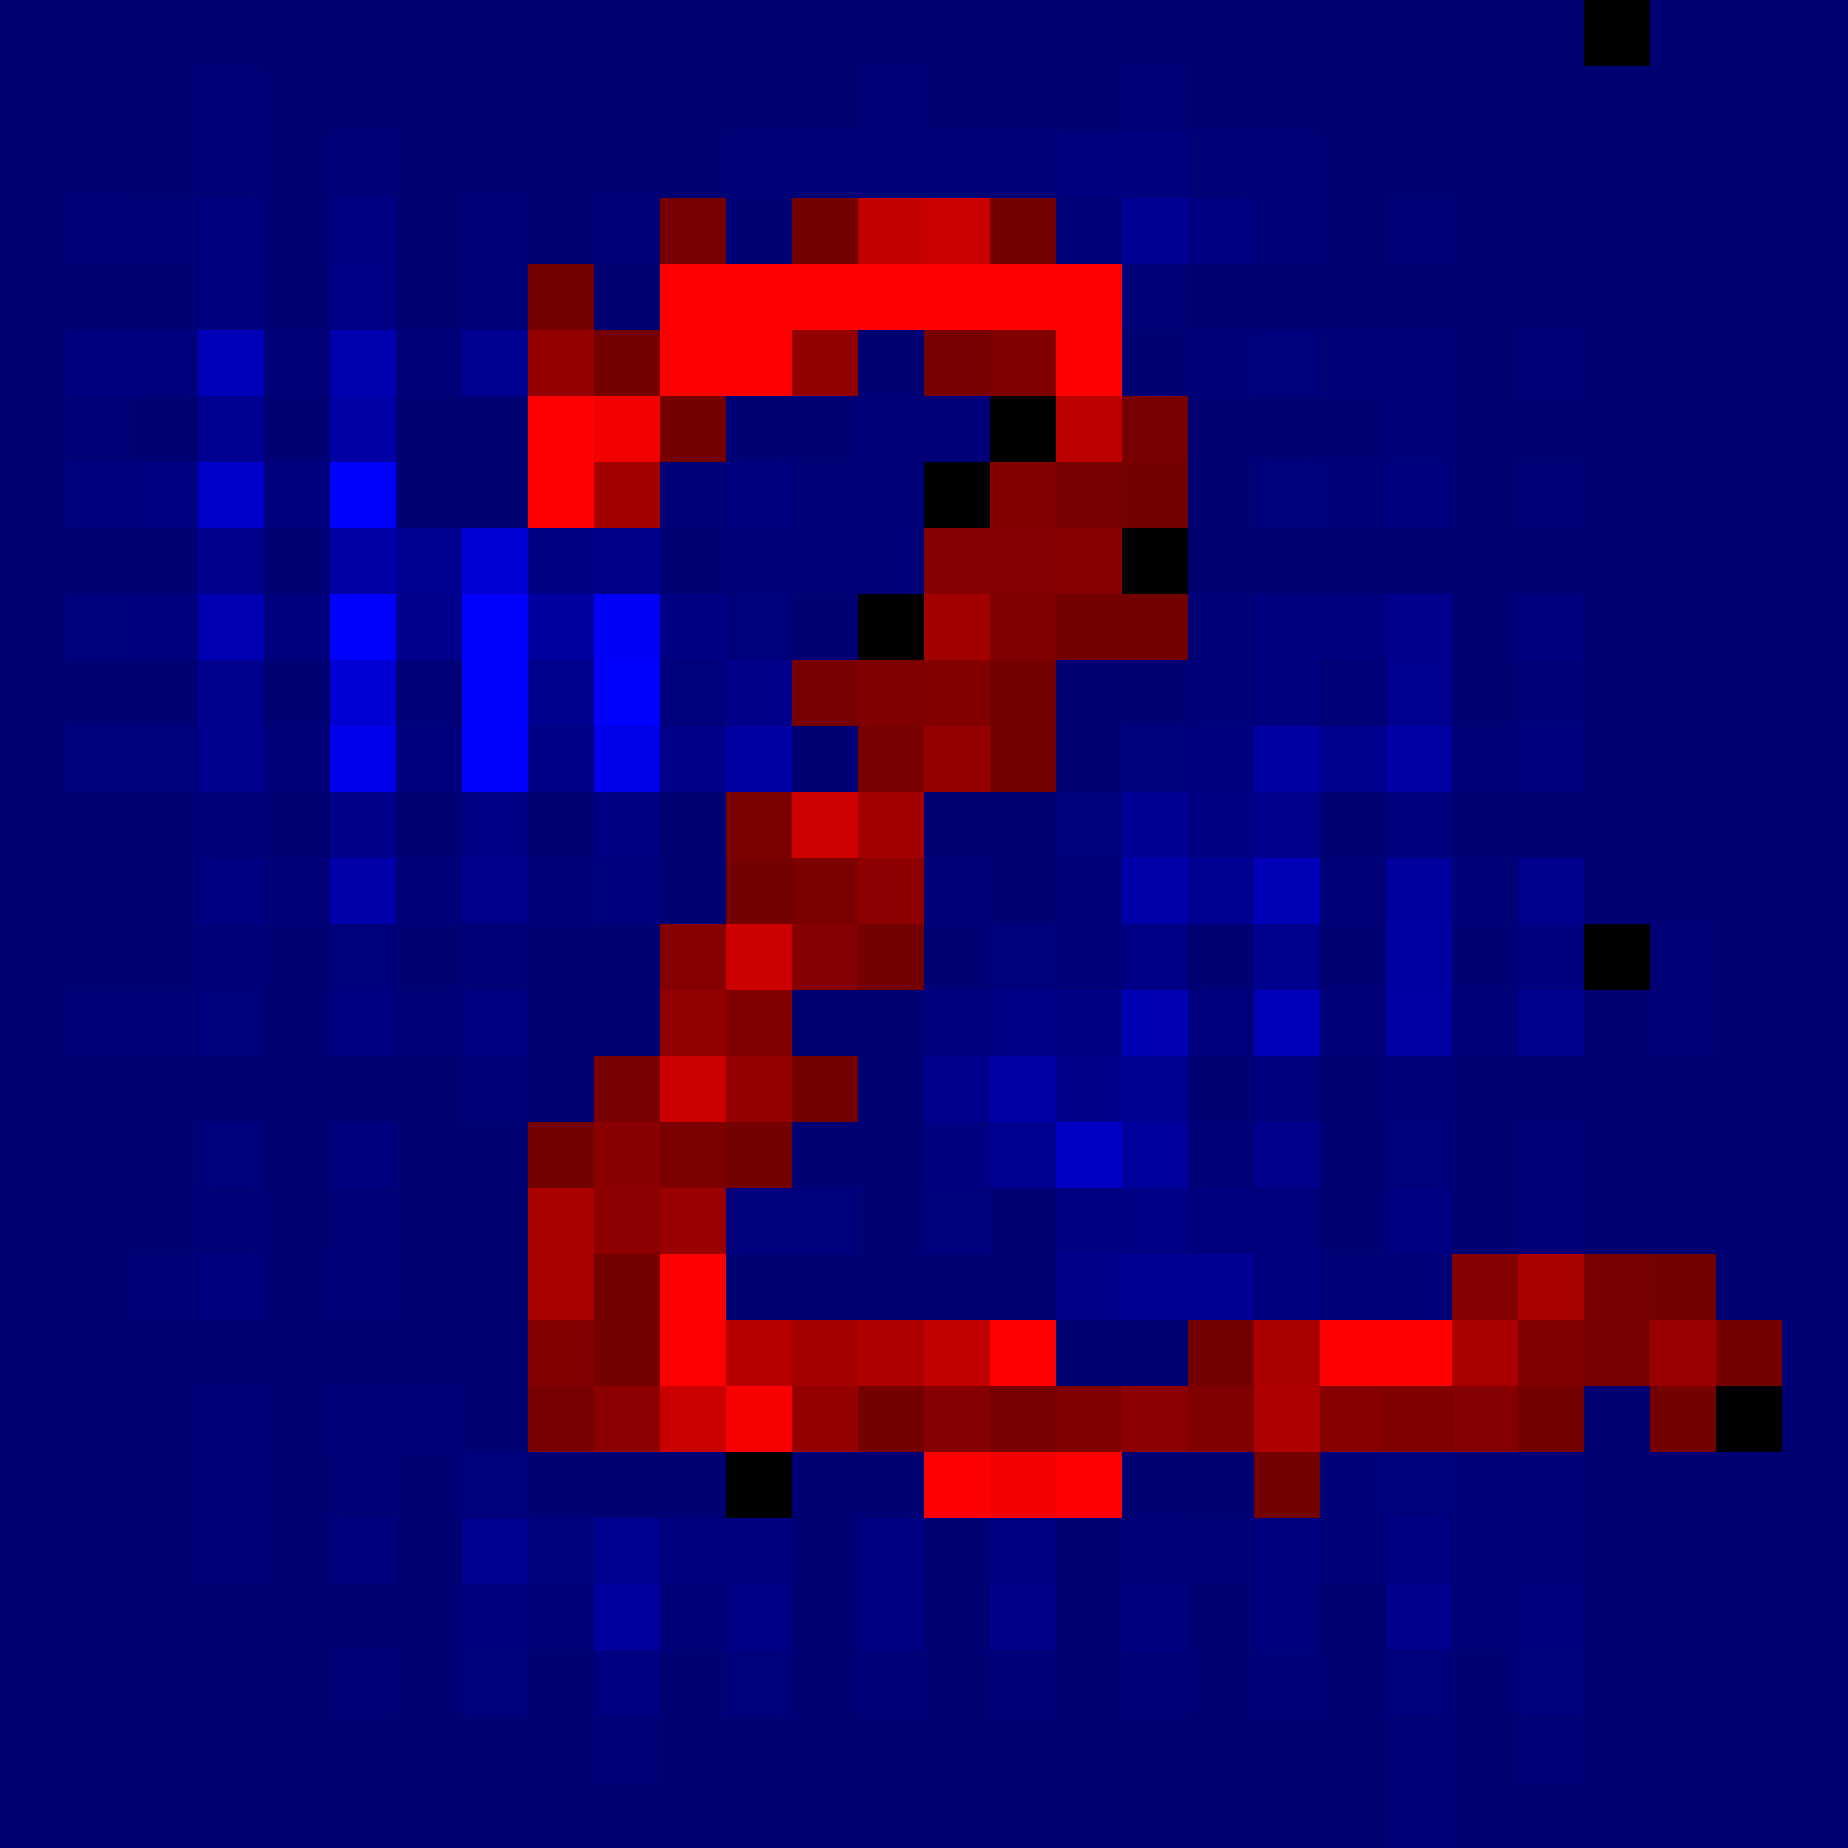
\includegraphics[width=\textwidth]{figures/mnist_ic_saliency/saliency_threshold_wrt_2_bright.png}
    \end{subfigure}
    \begin{subfigure}[b]{0.09\textwidth}
        \centering
        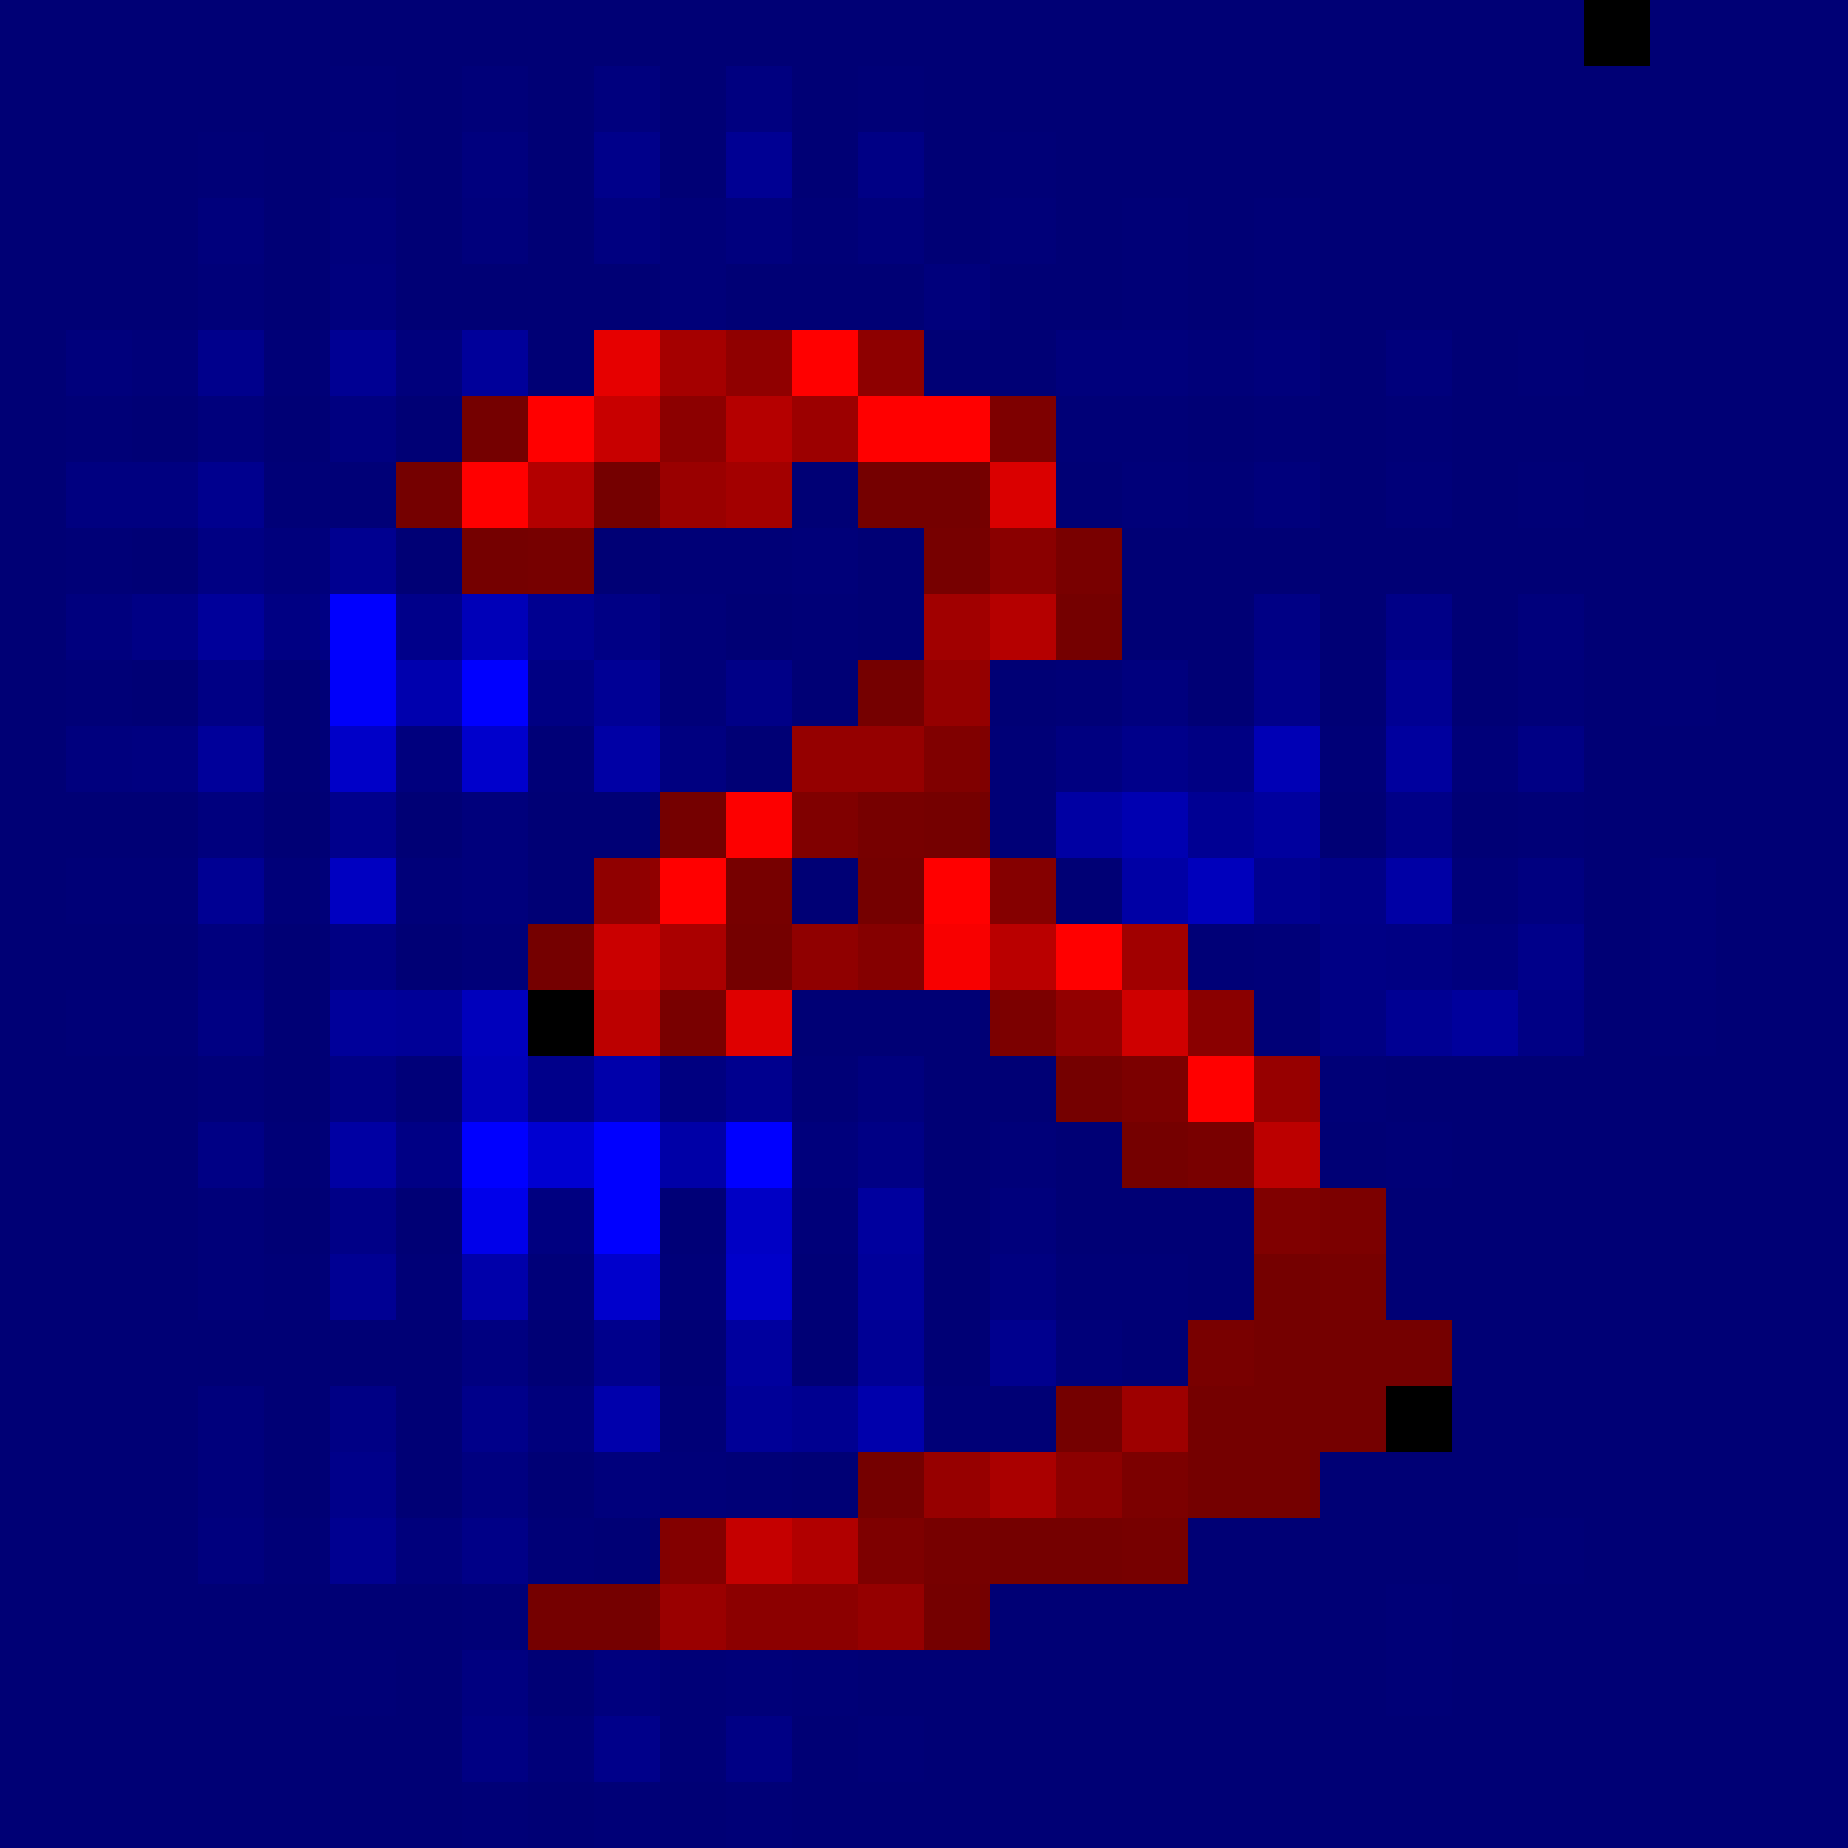
\includegraphics[width=\textwidth]{figures/mnist_ic_saliency/saliency_threshold_wrt_3_bright.png}
    \end{subfigure}
    \begin{subfigure}[b]{0.09\textwidth}
        \centering
        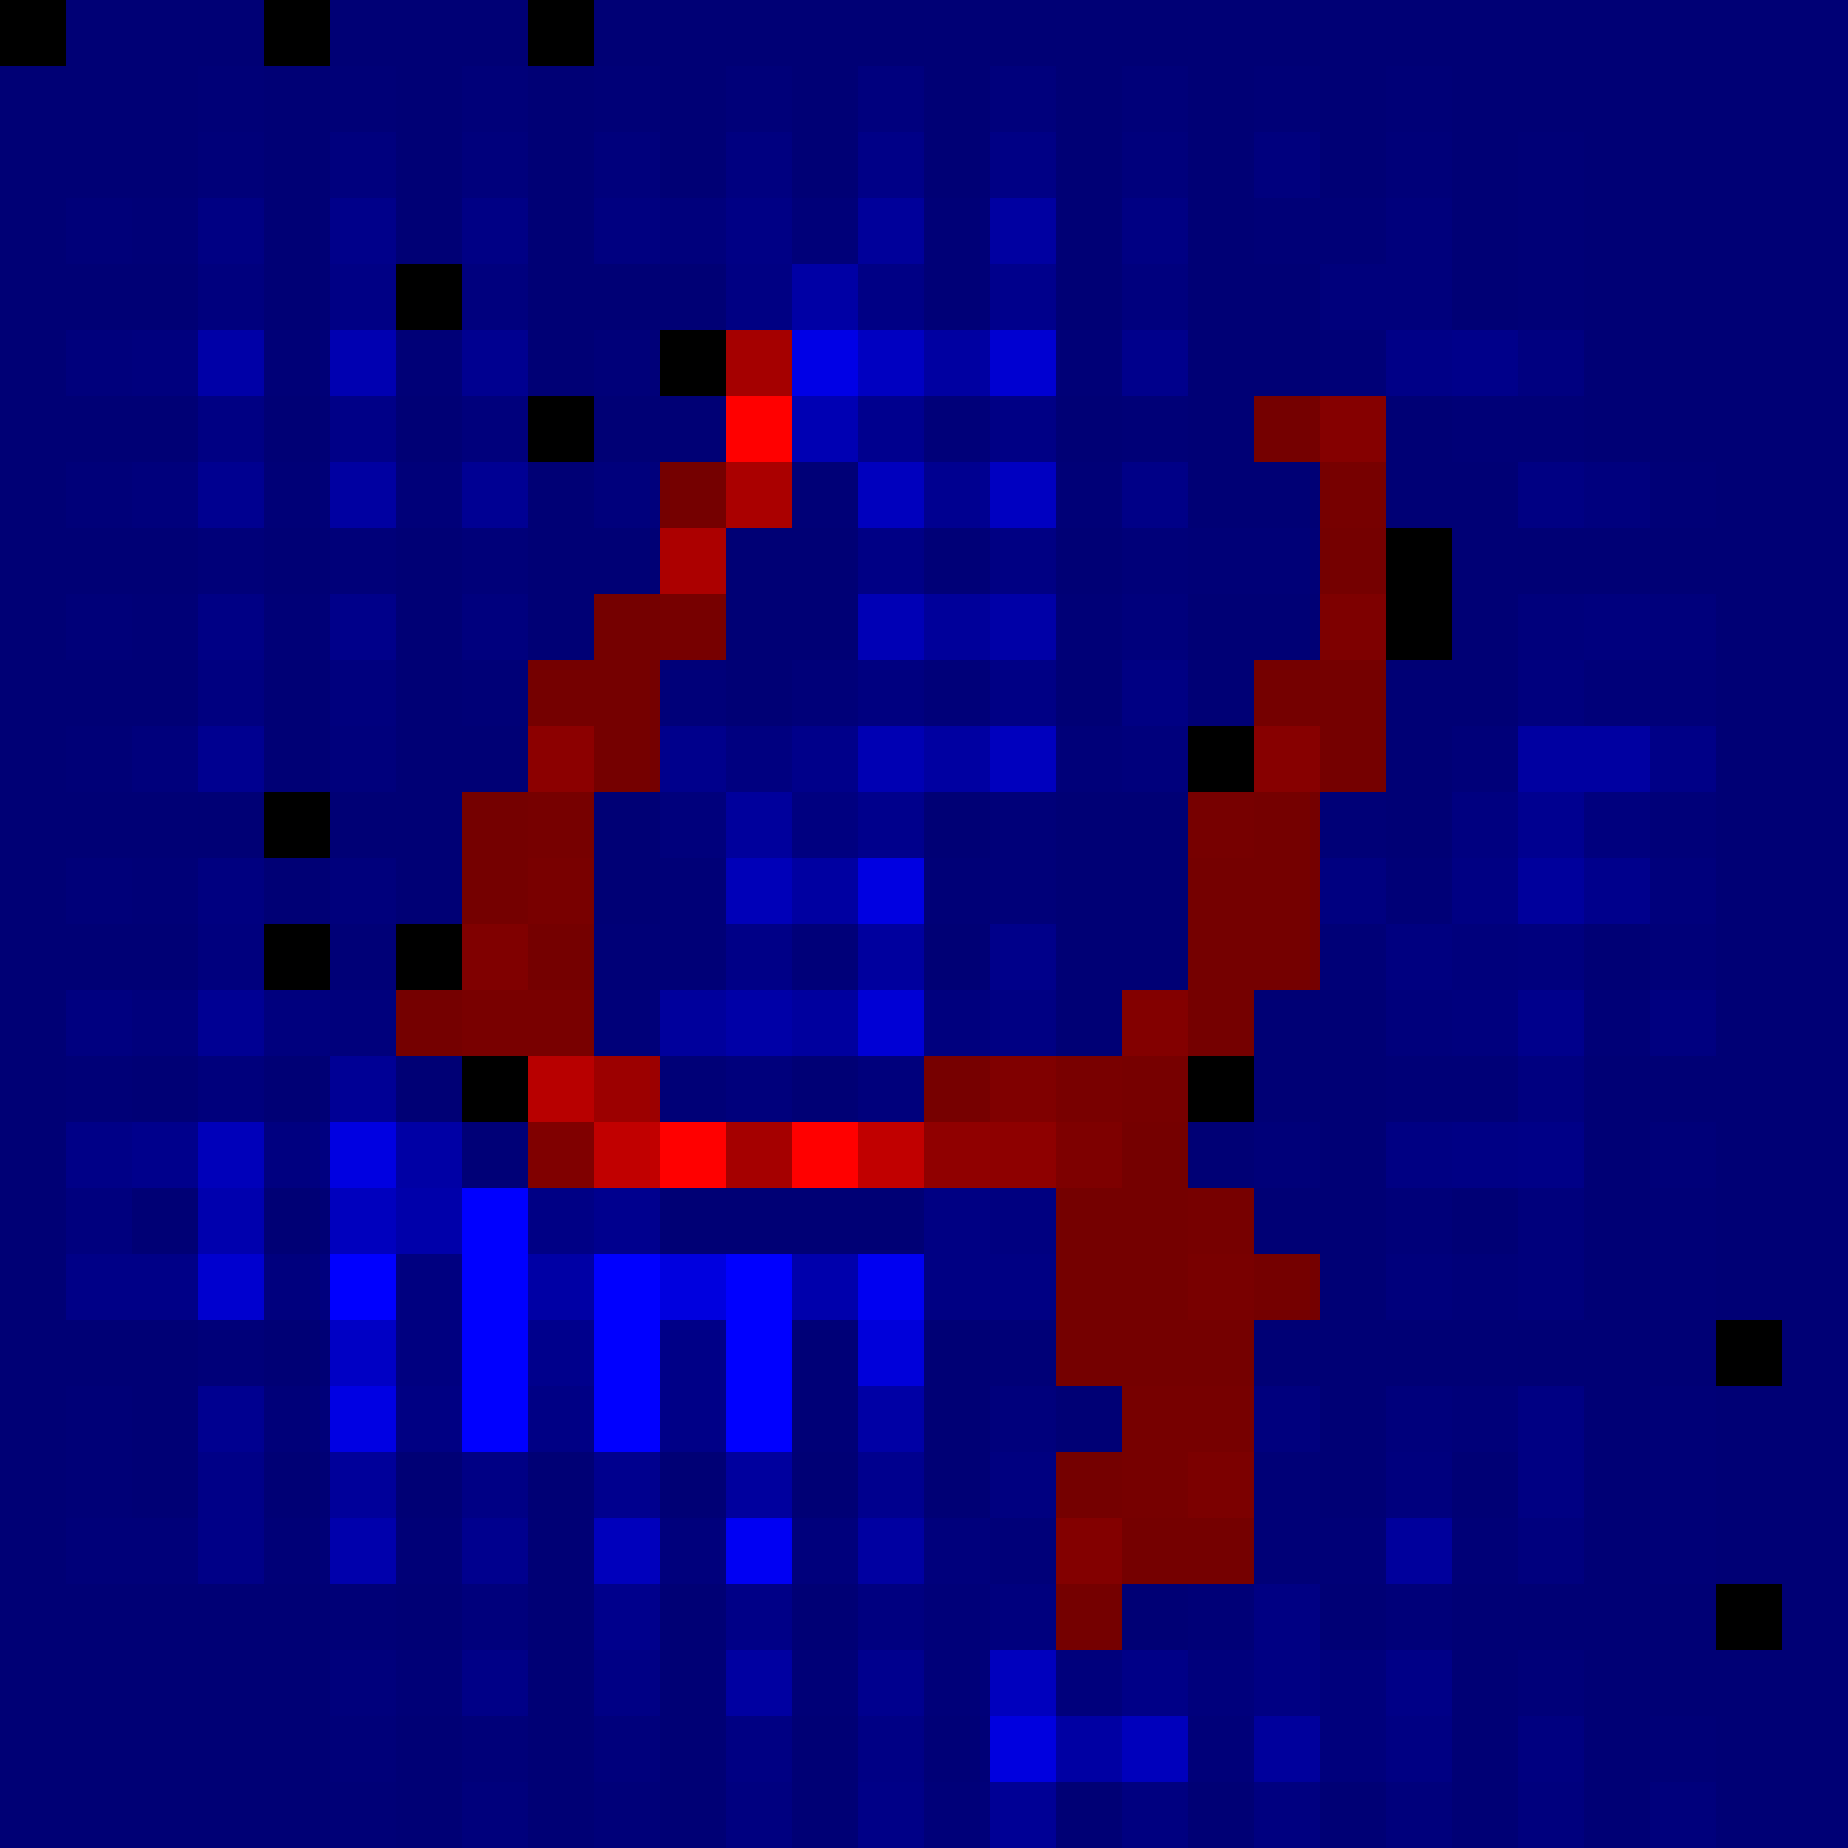
\includegraphics[width=\textwidth]{figures/mnist_ic_saliency/saliency_threshold_wrt_4_bright.png}
    \end{subfigure}
    \begin{subfigure}[b]{0.09\textwidth}
        \centering
        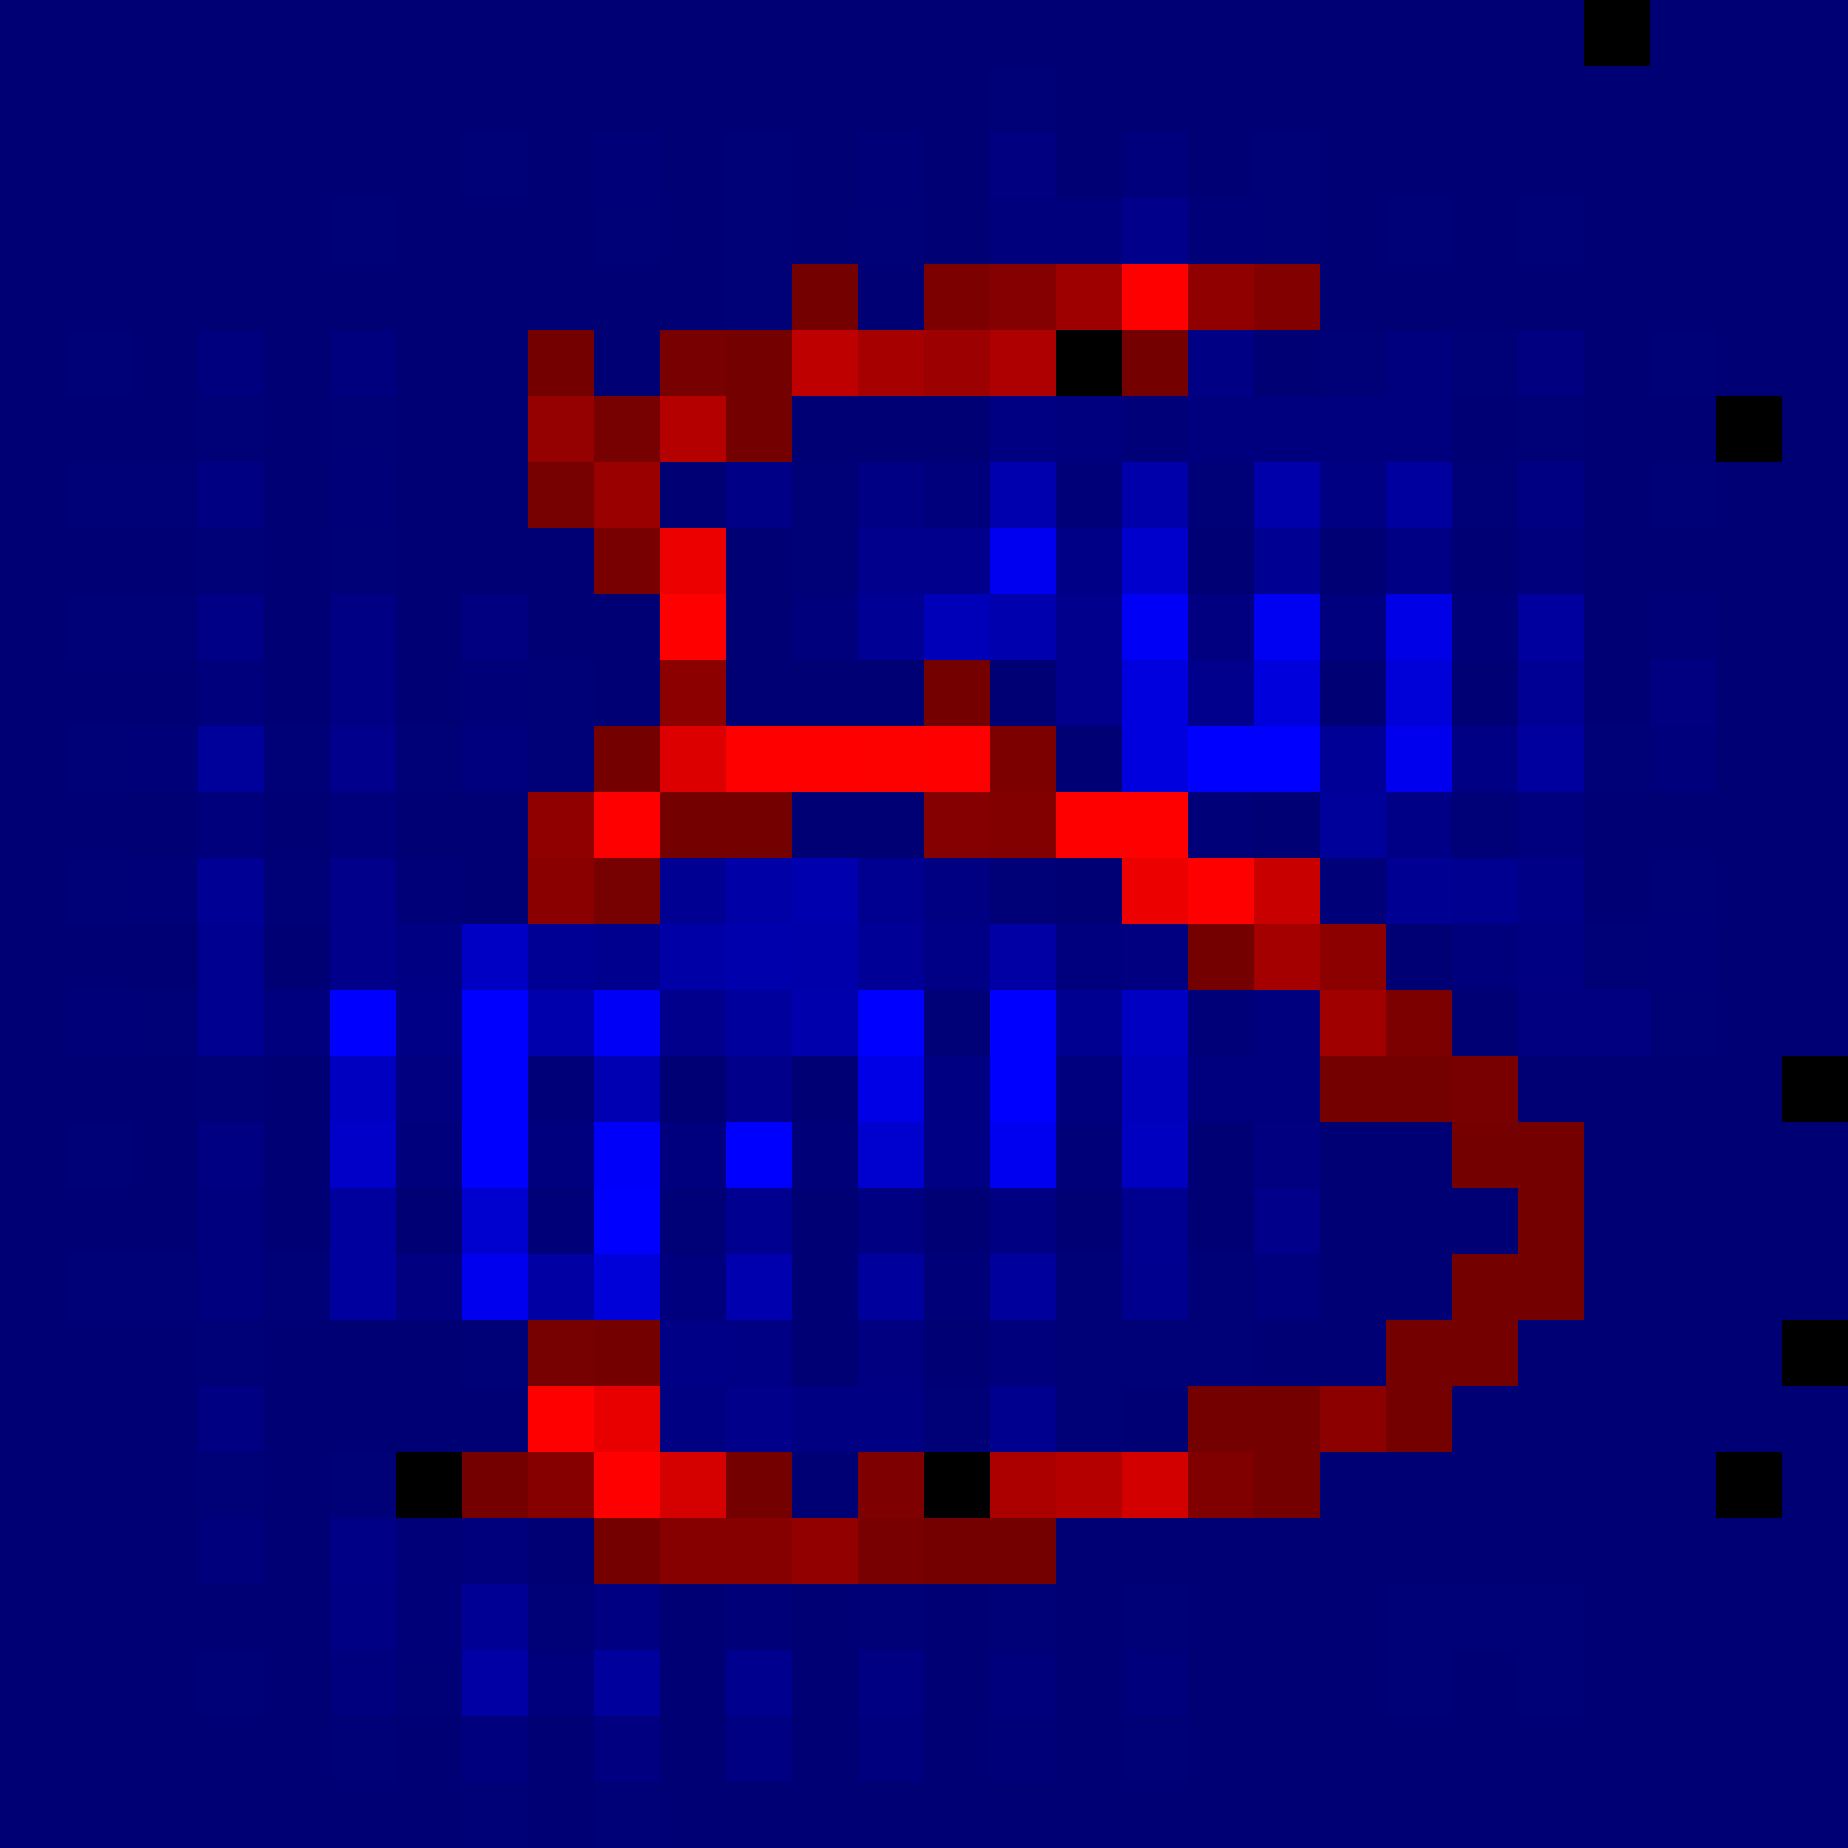
\includegraphics[width=\textwidth]{figures/mnist_ic_saliency/saliency_threshold_wrt_5_bright.png}
    \end{subfigure}
    \begin{subfigure}[b]{0.09\textwidth}
        \centering
        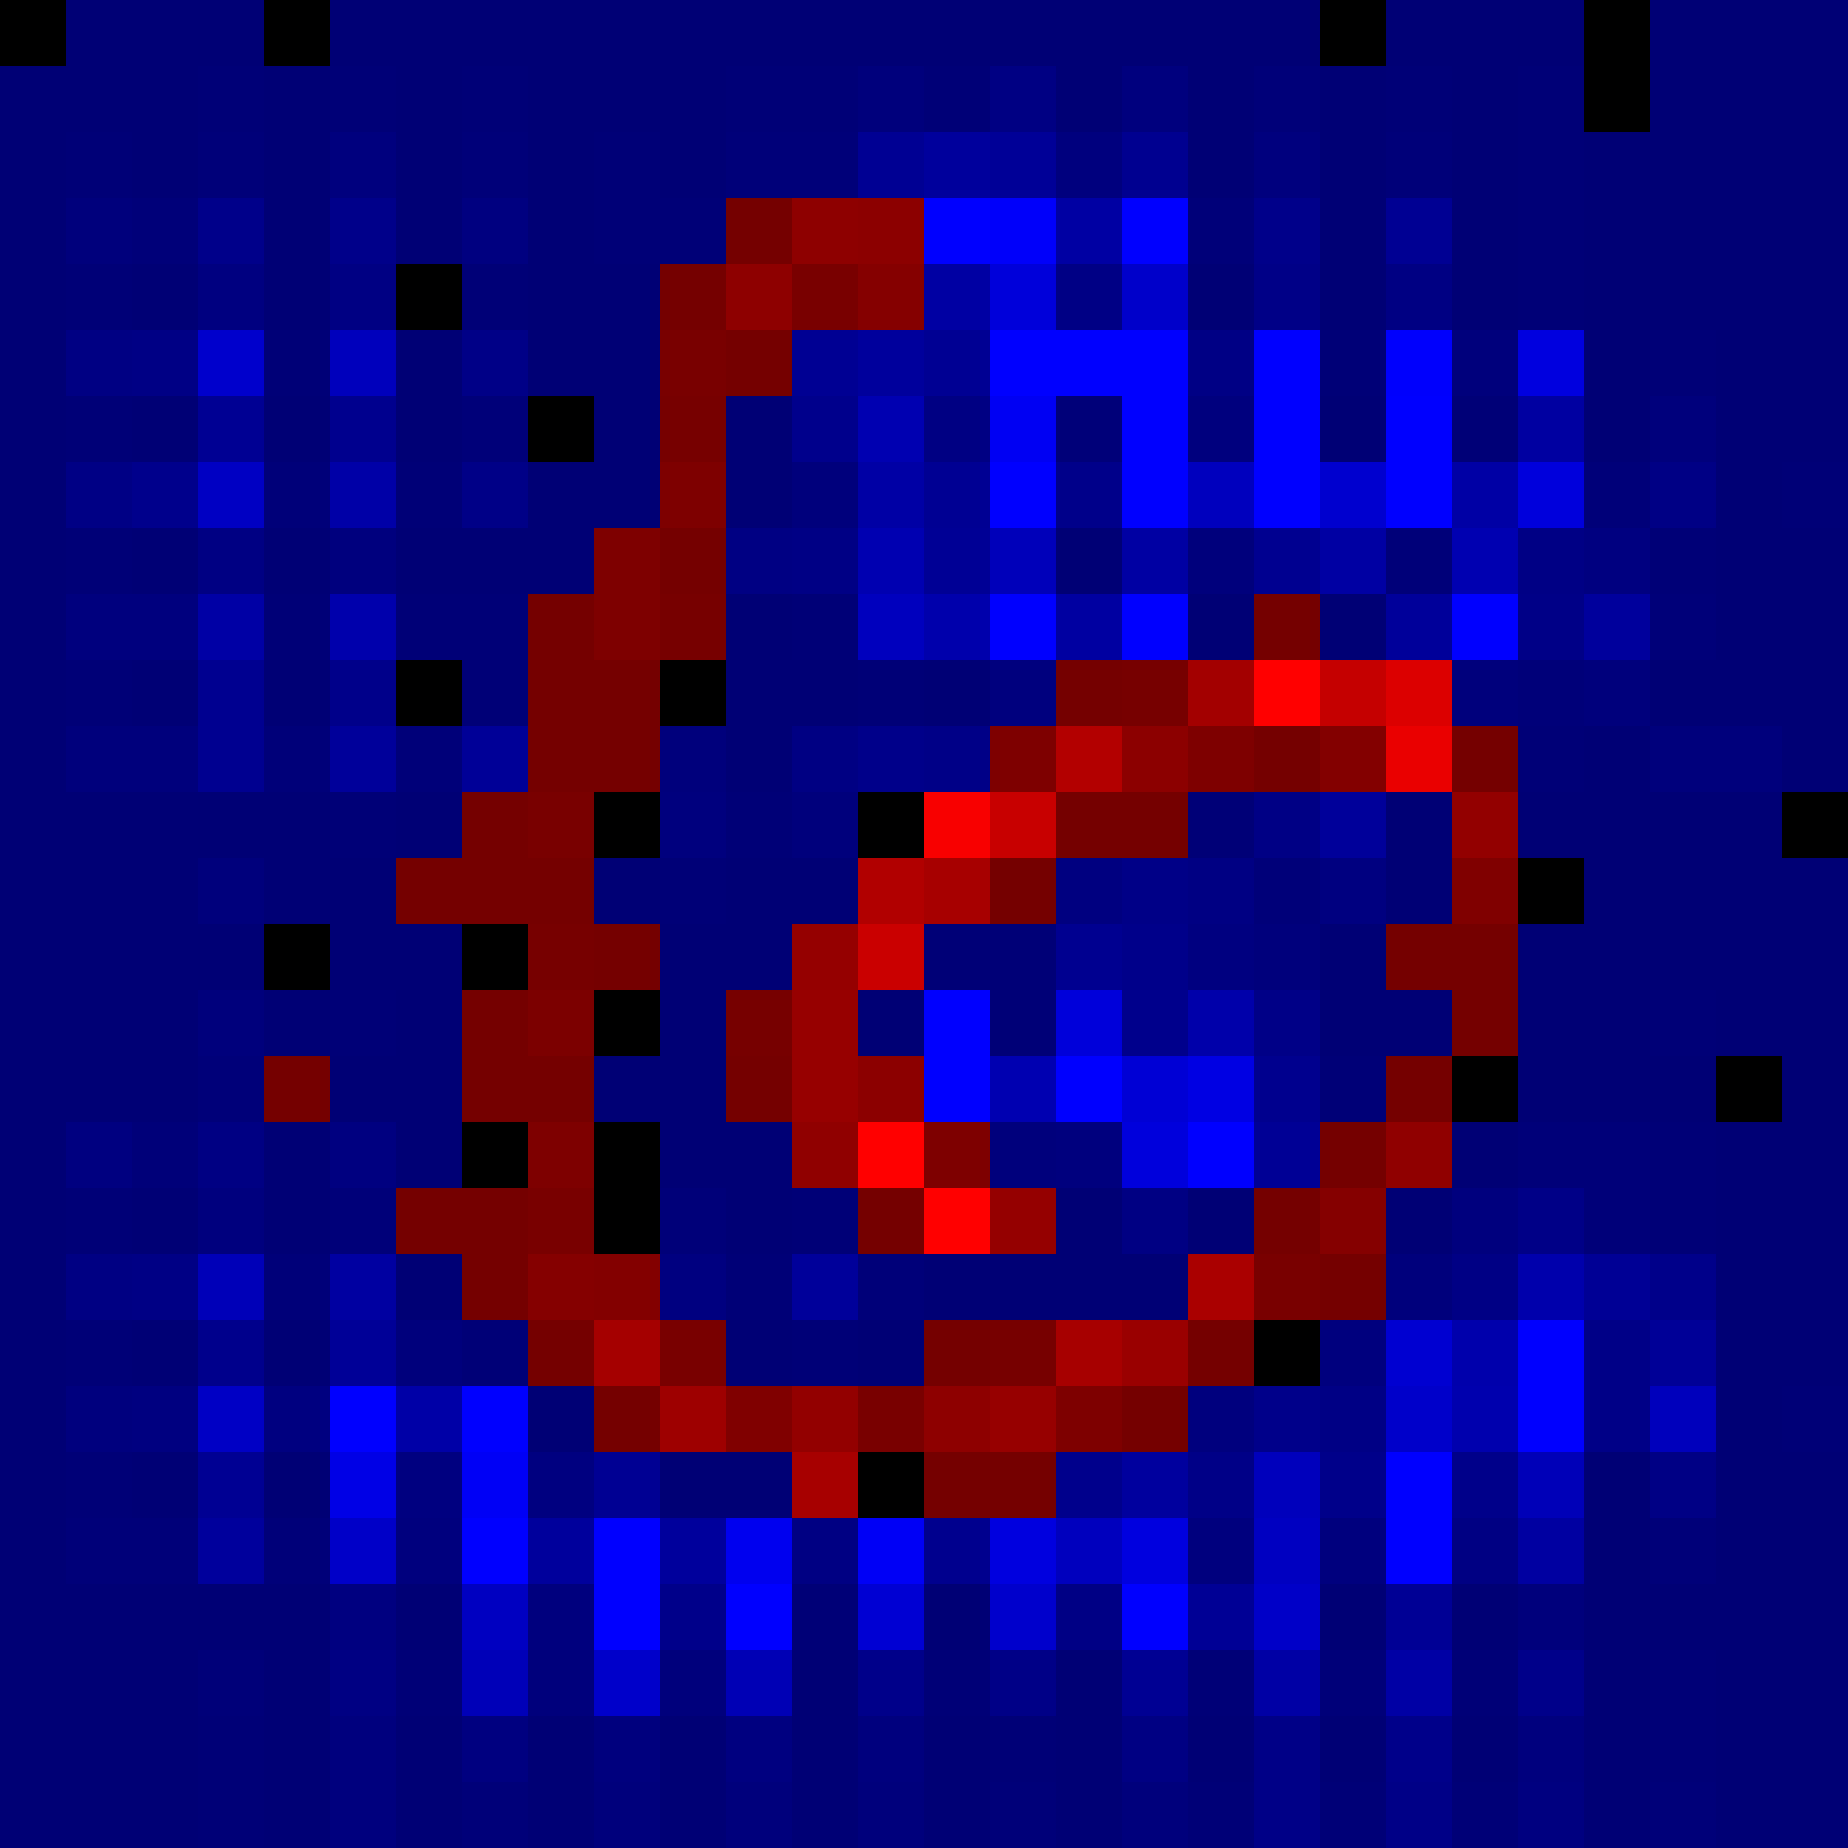
\includegraphics[width=\textwidth]{figures/mnist_ic_saliency/saliency_threshold_wrt_6_bright.png}
    \end{subfigure}
    \begin{subfigure}[b]{0.09\textwidth}
        \centering
        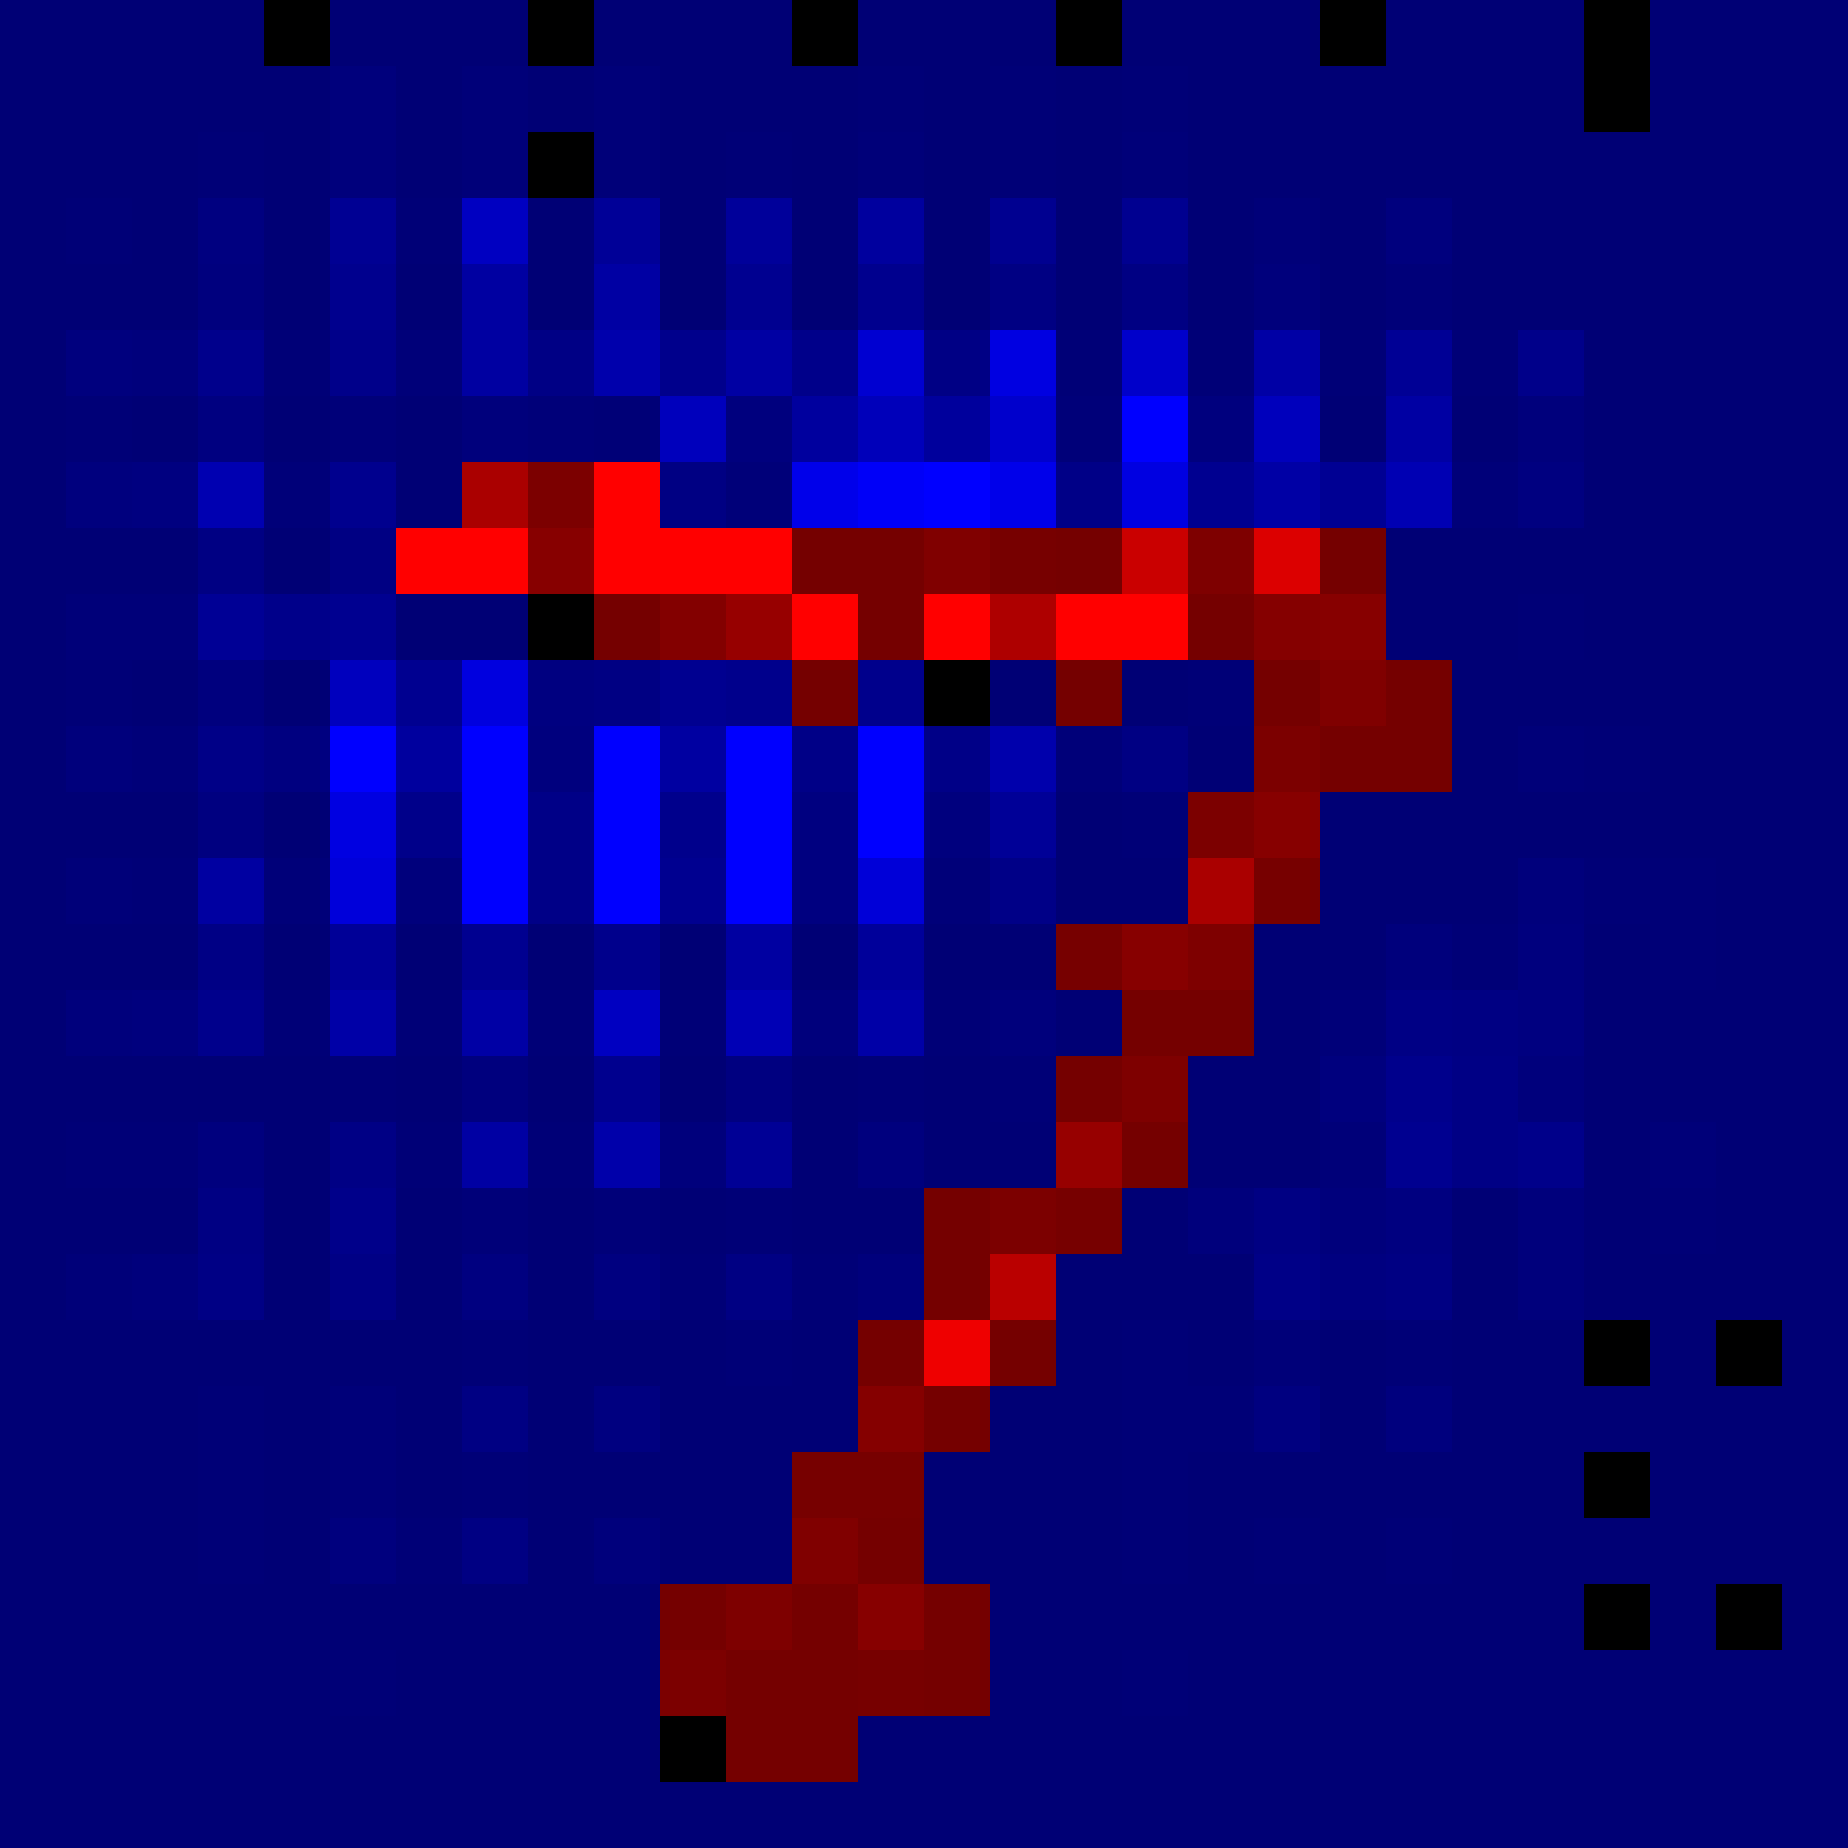
\includegraphics[width=\textwidth]{figures/mnist_ic_saliency/saliency_threshold_wrt_7_bright.png}
    \end{subfigure}
    \begin{subfigure}[b]{0.09\textwidth}
        \centering
        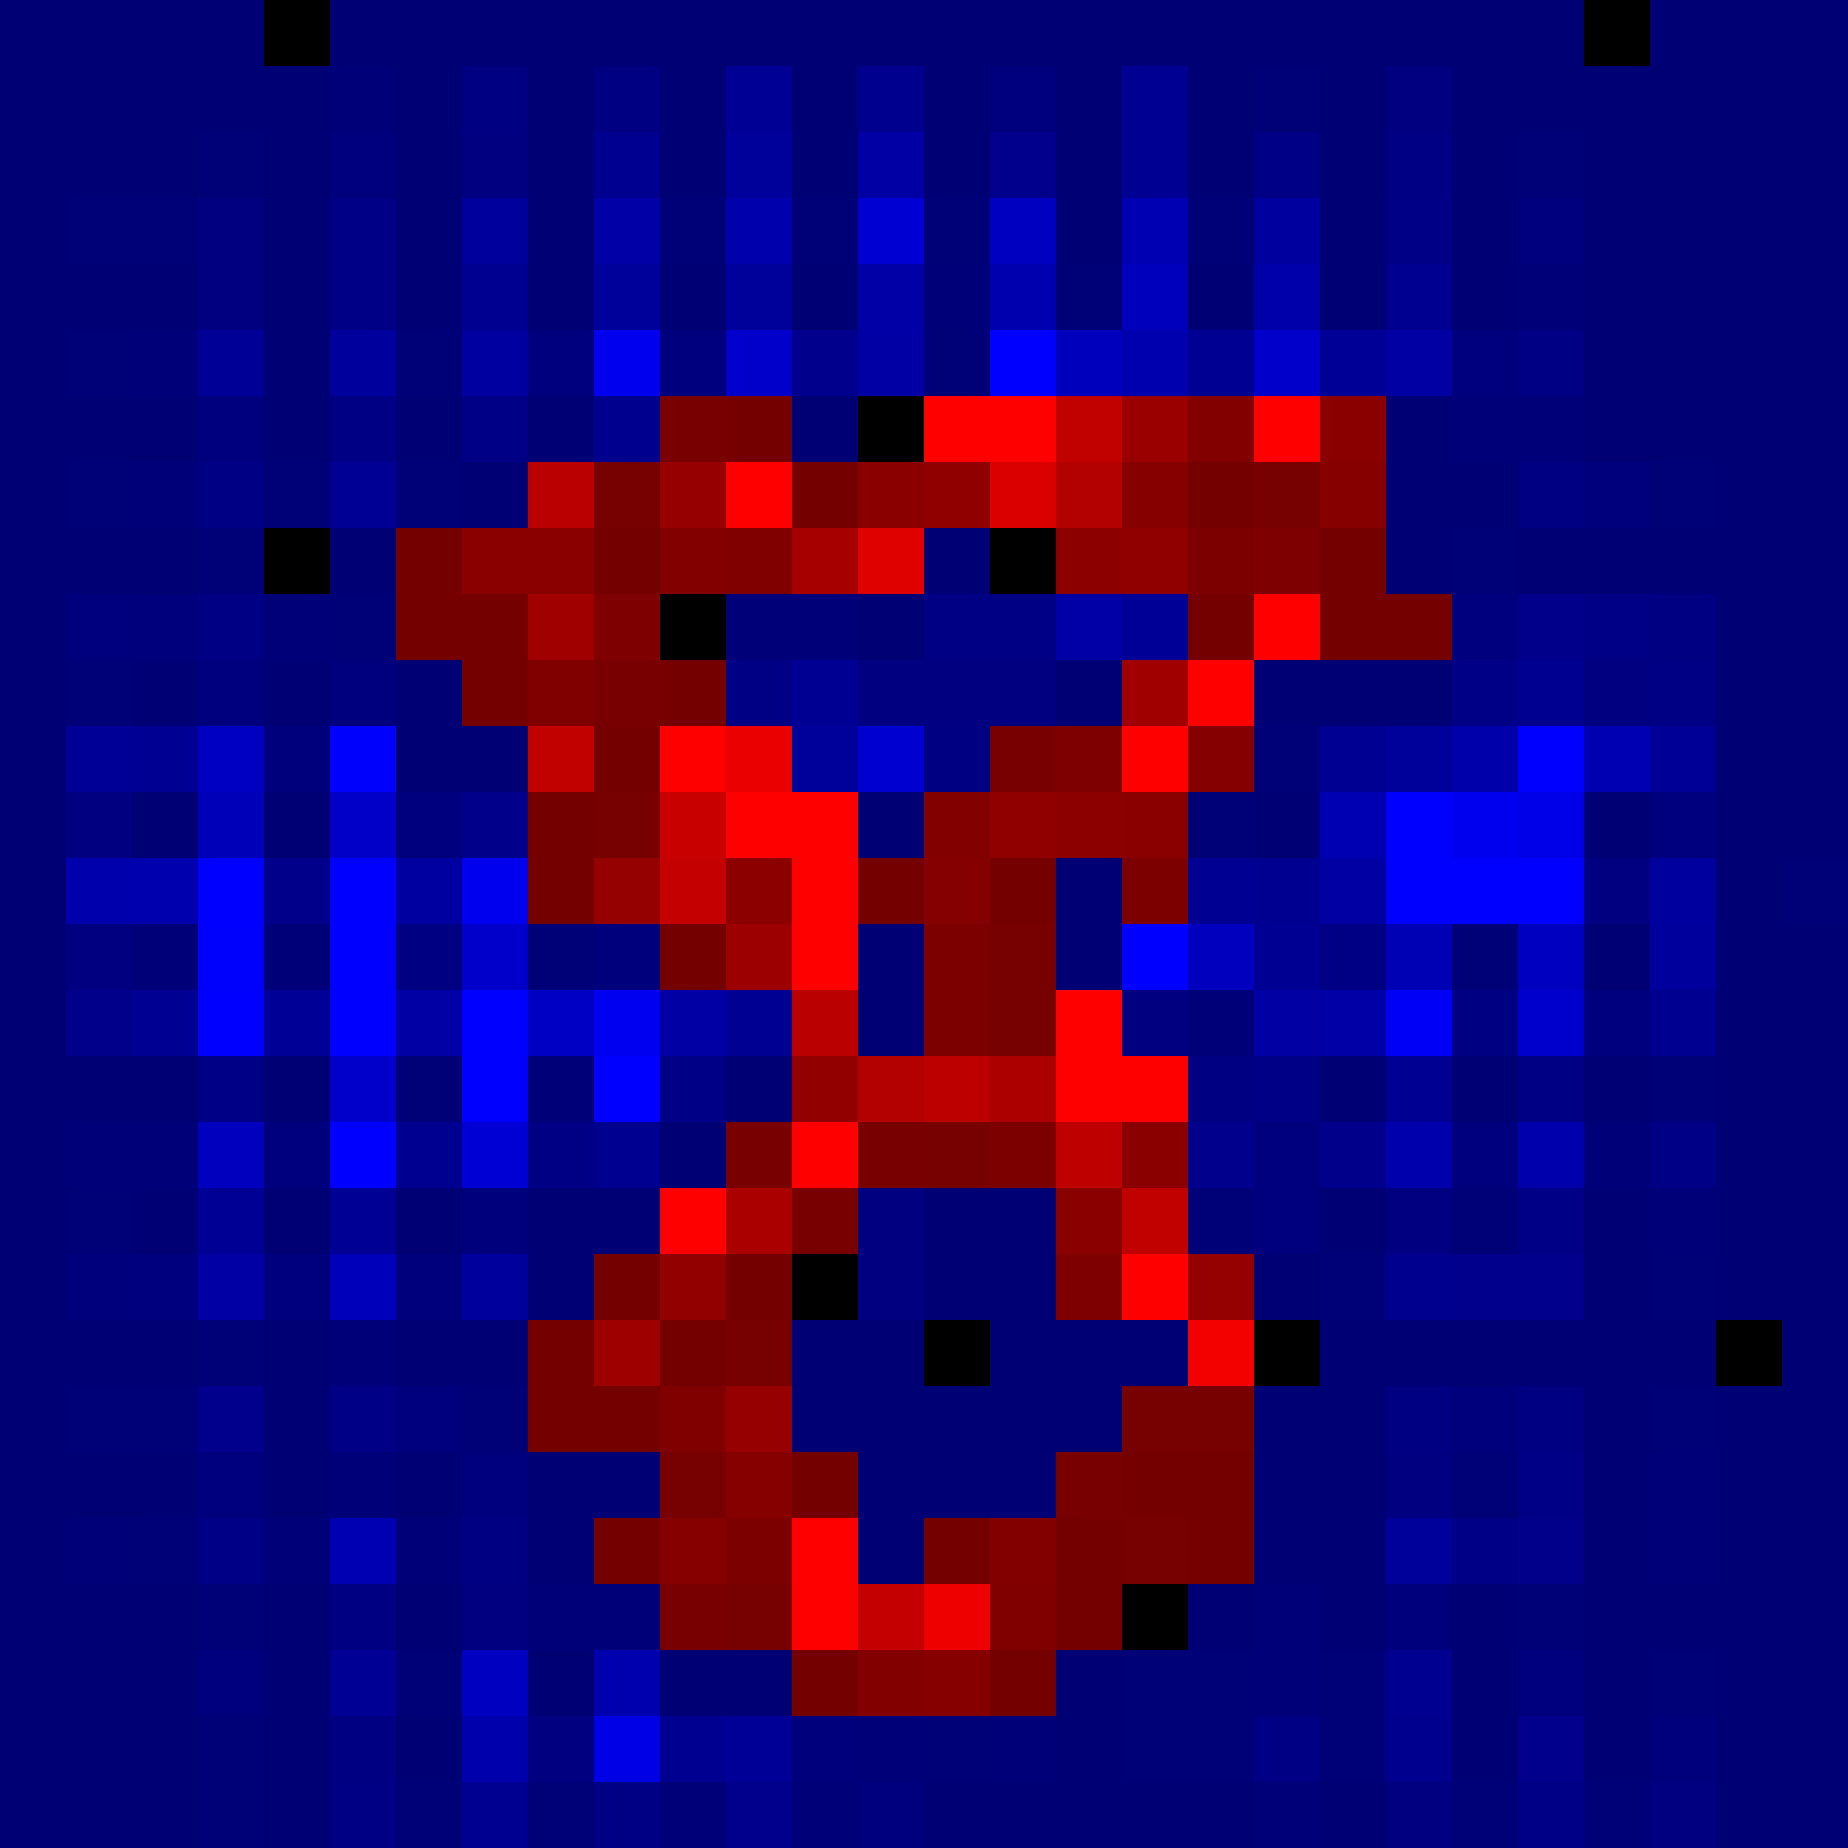
\includegraphics[width=\textwidth]{figures/mnist_ic_saliency/saliency_threshold_wrt_8_bright.png}
    \end{subfigure}
    \begin{subfigure}[b]{0.09\textwidth}
        \centering
        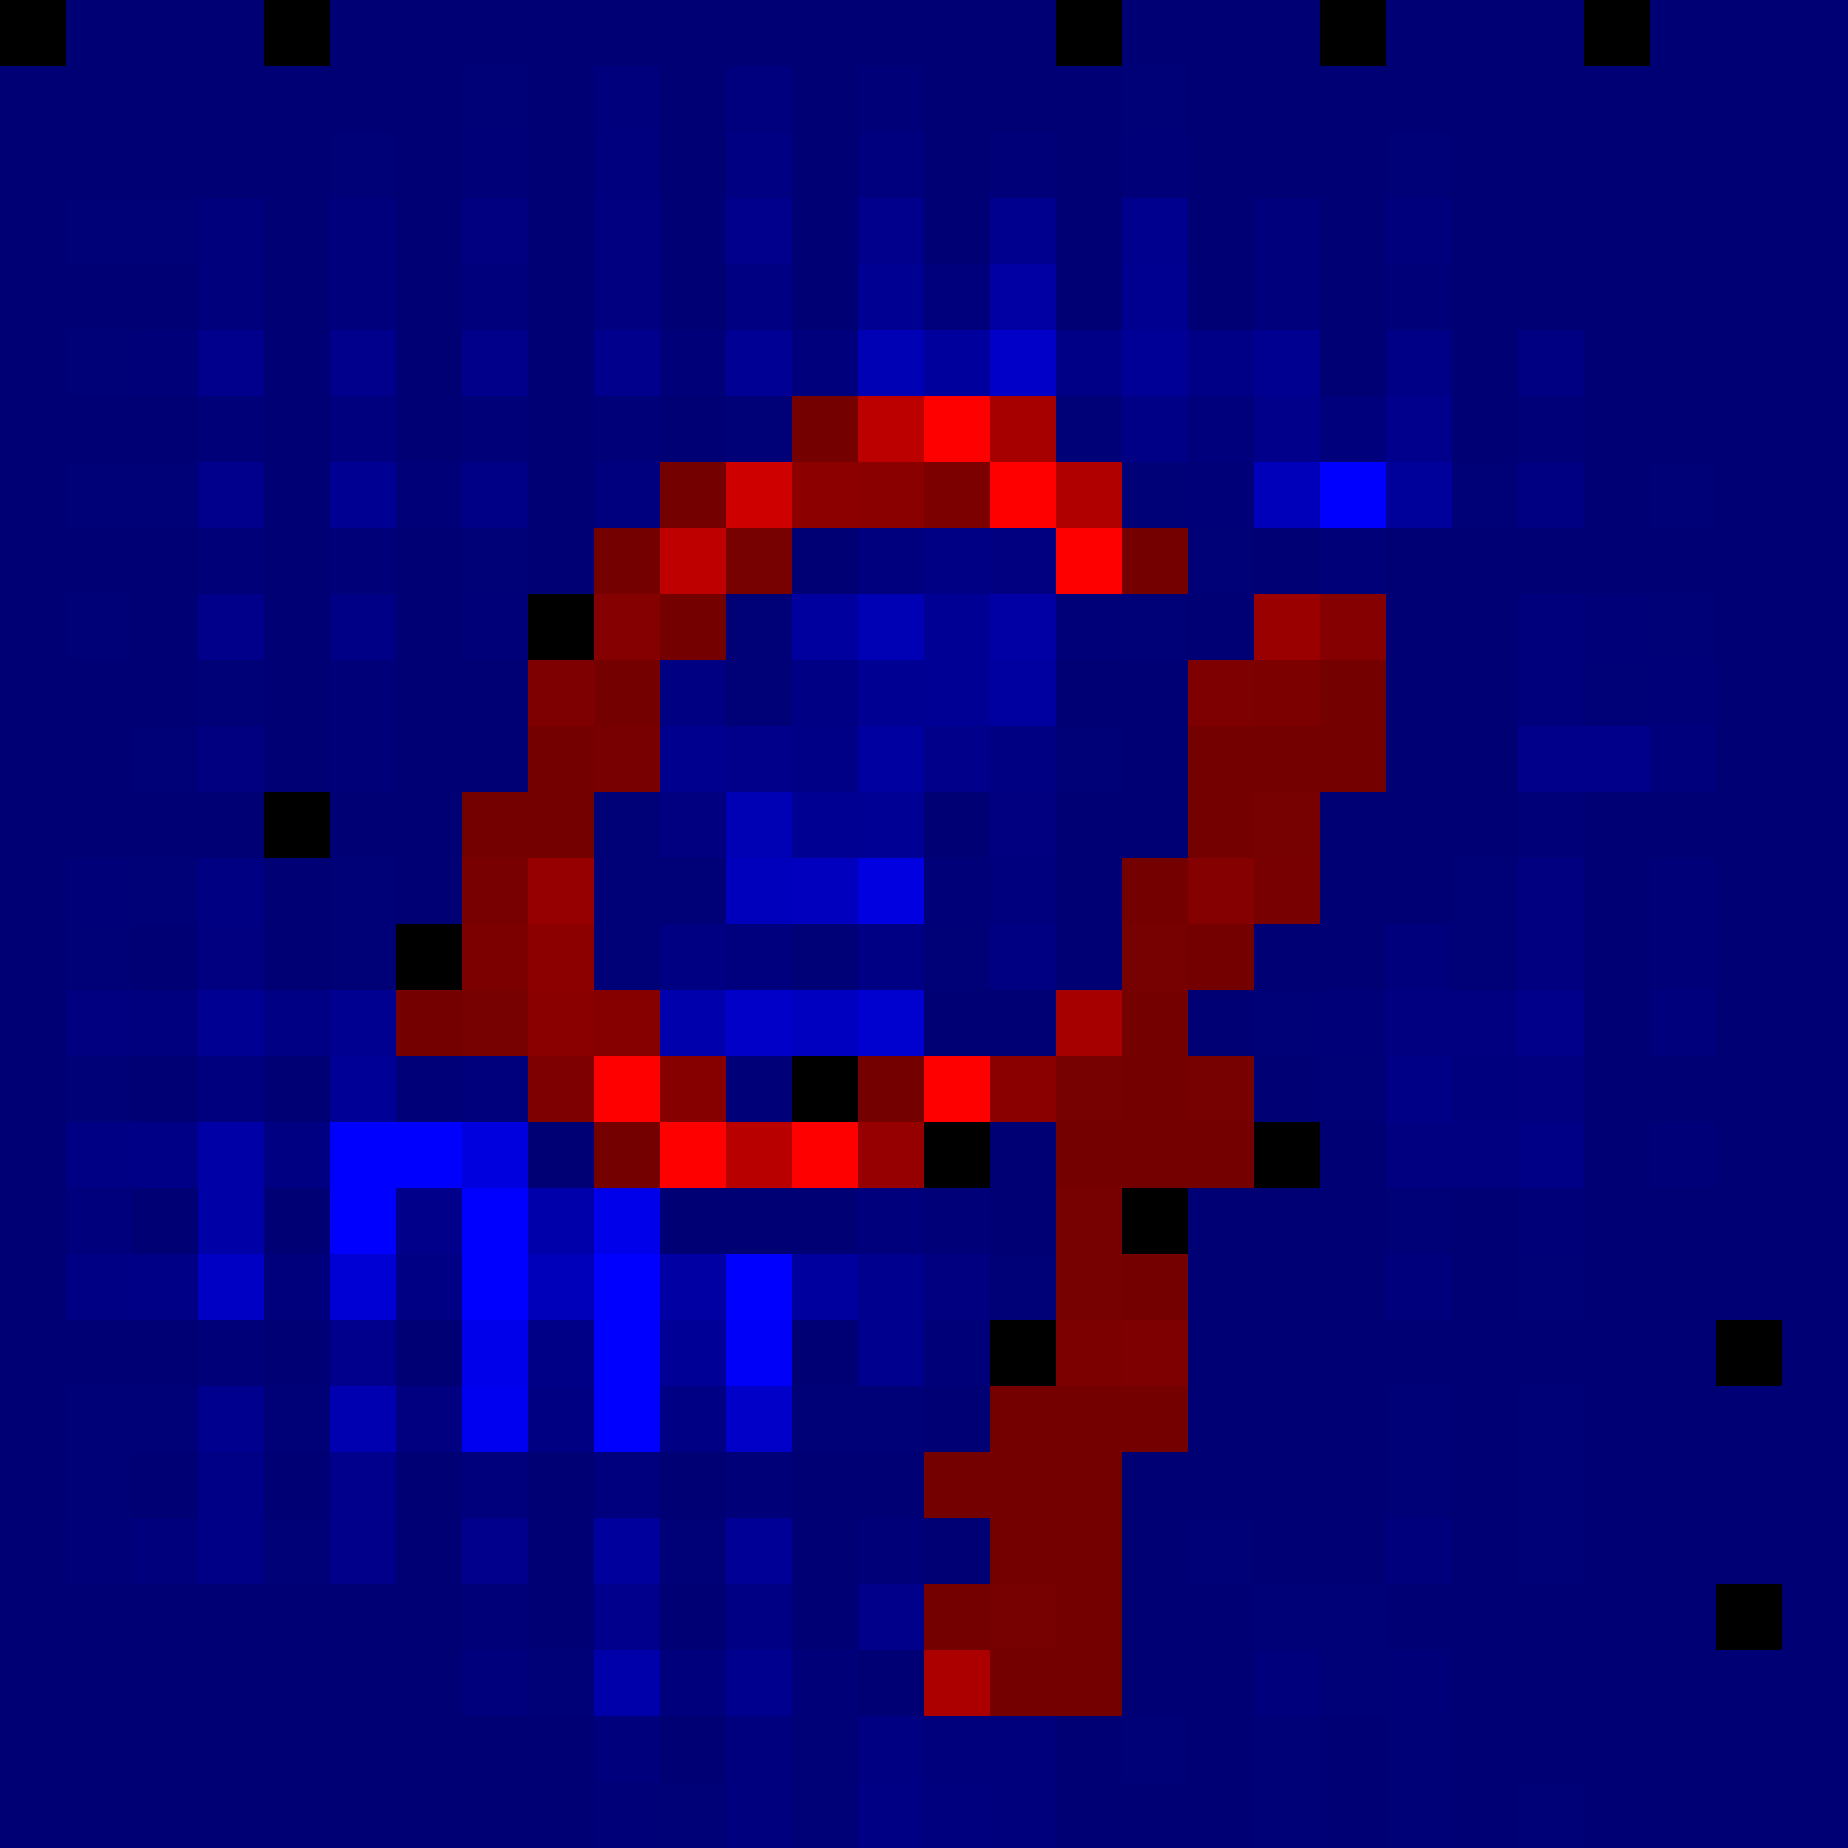
\includegraphics[width=\textwidth]{figures/mnist_ic_saliency/saliency_threshold_wrt_9_bright.png}
    \end{subfigure}

    \vspace{0.5cm}

    \begin{subfigure}[b]{0.09\textwidth}
        \centering
        
\includegraphics[width=\textwidth]{figures/mnist_ic_saliency/original_0.png}
        \caption*{\scriptsize Label 0}
    \end{subfigure}
    \begin{subfigure}[b]{0.09\textwidth}
        \centering
        
\includegraphics[width=\textwidth]{figures/mnist_ic_saliency/original_1.png}
        \caption*{\scriptsize Label 1}
    \end{subfigure}
    \begin{subfigure}[b]{0.09\textwidth}
        \centering
        
\includegraphics[width=\textwidth]{figures/mnist_ic_saliency/original_2.png}
        \caption*{\scriptsize Label 2}
    \end{subfigure}
    \begin{subfigure}[b]{0.09\textwidth}
        \centering
        
\includegraphics[width=\textwidth]{figures/mnist_ic_saliency/original_3.png}
        \caption*{\scriptsize Label 3}
    \end{subfigure}
    \begin{subfigure}[b]{0.09\textwidth}
        \centering
        
\includegraphics[width=\textwidth]{figures/mnist_ic_saliency/original_4.png}
        \caption*{\scriptsize Label 4}
    \end{subfigure}
    \begin{subfigure}[b]{0.09\textwidth}
        \centering
        
\includegraphics[width=\textwidth]{figures/mnist_ic_saliency/original_5.png}
        \caption*{\scriptsize Label 5}
    \end{subfigure}
    \begin{subfigure}[b]{0.09\textwidth}
        \centering
        
\includegraphics[width=\textwidth]{figures/mnist_ic_saliency/original_6.png}
        \caption*{\scriptsize Label 6}
    \end{subfigure}
    \begin{subfigure}[b]{0.09\textwidth}
        \centering
        
\includegraphics[width=\textwidth]{figures/mnist_ic_saliency/original_7.png}
        \caption*{\scriptsize Label 7}
    \end{subfigure}
    \begin{subfigure}[b]{0.09\textwidth}
        \centering
        
\includegraphics[width=\textwidth]{figures/mnist_ic_saliency/original_8.png}
        \caption*{\scriptsize Label 8}
    \end{subfigure}
    \begin{subfigure}[b]{0.09\textwidth}
        \centering
        
\includegraphics[width=\textwidth]{figures/mnist_ic_saliency/original_9.png}
        \caption*{\scriptsize Label 9}
    \end{subfigure}
    \caption{Input gradient visualizations of the \texttt{cnn\_maxout} IC model of ten digits with respect to their ground truth label. Top row: saliency maps. Bottom row: original images for each label. We colored positive and negative split-stream gradient values above threshold 0.2 red and blue respectively, where we colorized the ranking of the absolute values with an exponential decay.}

    \label{fig:mnist_ic_saliency}
\end{figure}
